\documentclass[a4paper,12pt]{article} % добавить leqno в [] для нумерации слева
\usepackage[a4paper,top=1.3cm,bottom=2cm,left=1.5cm,right=1.5cm,marginparwidth=0.75cm]{geometry}
%%% Работа с русским языком
\usepackage{cmap}					% поиск в PDF
\usepackage{mathtext} 				% русские буквы в фомулах
\usepackage[T2A]{fontenc}			% кодировка
\usepackage[utf8]{inputenc}			% кодировка исходного текста
\usepackage[english,russian]{babel}	% локализация и переносы
\usepackage{multirow}

\usepackage{graphicx}

\usepackage{wrapfig}
\usepackage{tabularx}

\usepackage{hyperref}
\usepackage[rgb]{xcolor}
\hypersetup{
colorlinks=true,urlcolor=blue
}

%%% Дополнительная работа с математикой
\usepackage{amsmath,amsfonts,amssymb,amsthm,mathtools} % AMS
\usepackage{icomma} % "Умная" запятая: $0,2$ --- число, $0, 2$ --- перечисление

%% Номера формул
\mathtoolsset{showonlyrefs=true} % Показывать номера только у тех формул, на которые есть \eqref{} в тексте.

%% Шрифты
\usepackage{euscript}	 % Шрифт Евклид
\usepackage{mathrsfs} % Красивый матшрифт

%% Свои команды
\DeclareMathOperator{\sgn}{\mathop{sgn}}

%% Перенос знаков в формулах (по Львовскому)
\newcommand*{\hm}[1]{#1\nobreak\discretionary{}
{\hbox{$\mathsurround=0pt #1$}}{}}

%% Графики
\usepackage{tikz}
\usepackage{pgfplots}
\pgfplotsset{compat=1.9}

\usepackage{subcaption}

\date{\today}

\begin{document}

\begin{titlepage}
	\begin{center}
		{\large МОСКОВСКИЙ ФИЗИКО-ТЕХНИЧЕСКИЙ ИНСТИТУТ (НАЦИОНАЛЬНЫЙ ИССЛЕДОВАТЕЛЬСКИЙ УНИВЕРСИТЕТ)}
	\end{center}
	\begin{center}
		{\large Физтех-школа прикладной математики и информатики}
	\end{center}
	
	
	\vspace{4.5cm}
	{\huge
		\begin{center}
			{\bf Отчёт о выполнении лабораторной работы 3.6.1}\\
			Спектральный анализ электрических сигналов
		\end{center}
	}
	\vspace{1cm}
	\begin{center}
		{\large Соболевский Федор Александрович \\
			\vspace{0.2cm}
			Б05-111}
	\end{center}
	\vspace{8cm}
	\begin{center}
		Сентябрь 2022
	\end{center}
\end{titlepage}

\section{Аннотация}

В данной работе исследовано представление электрических сигналов различной формы в виде суммы гармонических сигналов разных частот. Исследованы спектры периодических прямоугольных сигналов, последовательностей цугов и амплитудно-модулированных сигналов. Коэффициенты в разложении сигналов определены экспериментально и теоретически. Полученные результаты сравнены, определены погрешности измерений и вычислений.

\section{Теоретические сведения}

\subsection{Разложение электрических сигналов на периодические колебания}

\subsubsection*{Разложение Фурье}

\par Спектральный анализ электрического сигнала - это представление его в виде суммы сигналов различных частот. Для этого используется разложение в ряд Фурье - представление функции в виде суммы гармонических функций.

Пусть задана функция $f(t)$, которая периодически повторяется с частотой $\omega_1 = \dfrac{2\pi}{T}$, где $T$ --- период повторения импульсов. Её разложение в ряд Фурье имеет вид 

\begin{equation}
    f(t) = \dfrac{a_0}{2} + \sum\limits_{n = 1}^{\infty}\left[a_n \cos \left(n \omega_1t\right) + b_n \sin \left(n \omega_1t\right)\right]
    \label{Fourier1}
\end{equation}

или

\begin{equation}
    f(t) = \dfrac{a_0}{2} + \sum\limits_{n = 1}^{\infty}A_n \cos \left(n\omega_1 t - \psi_n\right).
    \label{Fourier2}
\end{equation}

Если сигнал чётный относительно $t = 0$, в тригонометрической записи остаются только члены с косинусами, если нечетный - только члены с синусами.

Коэффициенты в формуле \eqref{Fourier1} определяются по формулам

\begin{equation}
\begin{array}{c}
    a_n = \dfrac{2}{T} \int\limits_{t_0}^{t_0 + T} f(t) \cos\left(n \omega_1 t\right) dt,\\
    \\
    b_n = \dfrac{2}{T} \int\limits_{t_0}^{t_0 + T} f(t) \sin\left(n \omega_1 t\right) dt.
\end{array}
\label{FourierKoeffs}
\end{equation}

Здесь $t_0$ --- время, с которого мы начинаем отсчет.

Связав формулы \eqref{Fourier1} и \eqref{Fourier2}, можно получить выражения для $A_n$  и $\psi_n$:

\begin{equation}
\begin{array}{l}
    A_n = \sqrt{a_n^2+b_n^2},\\
    \psi_n = \arctan \dfrac{b_n}{a_n}.
\end{array}
\end{equation}

\subsubsection*{Периодическая последовательность прямоугольных импульсов}

\begin{figure}[h]
    \centering
    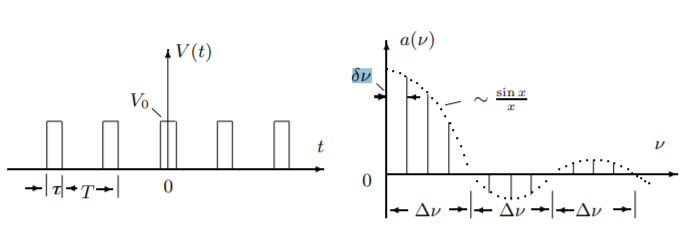
\includegraphics[width=0.8\textwidth]{2.png} 
    \caption{Последовательность прямоугольных импульсов и её спектр}
    \label{rectangularImpulses}
\end{figure}

Рассмотрим последовательность прямоугольных импульсов с циклической частотой $\omega_1 = \dfrac{2\pi}{T}$ и длительностью импульса $\tau$. Пусть $t = 0$ в середине импульса (см. рис. \ref{rectangularImpulses}). Исходя из \eqref{FourierKoeffs}, коэффициенты при косинусных составляющих будут равны

\begin{equation}
    a_n = \dfrac{2}{T} \int\limits_{-\tau/2}^{\tau/2} V_0 \cos\left(n\omega_1 t\right) dt = 2 V_0 \dfrac{\tau}{T} \dfrac{\sin\left(n\omega_1\tau/2\right)}{n\omega_1\tau/2} \sim \dfrac{\sin x}{x}.
\end{equation}

Здесь $V_0$ - амплитуда сигнала. Интеграл в данном случае можно брать только от $-\tau/2$ до $\tau/2$, так как в остальные моменты времени в пределах периода колебаний функция равна нулю. Поскольку функция задана чётной, $b_n = 0$. 

Пусть $T$ кратно $\tau$. Тогда введем ширину спектра, равную $\Delta \omega$ --- расстояние от главного максимума до первого нуля огибающей, возникающего при $n = \dfrac{2\pi}{\tau \omega_1}$. При этом

\begin{equation}
    \Delta \omega \tau \simeq 2\pi \Rightarrow \Delta \nu \Delta t \simeq 1.
\end{equation}

\subsubsection*{Периодическая последовательность цугов}

\begin{figure}[h]
    \centering
    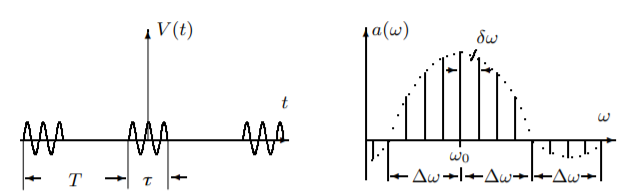
\includegraphics[width=0.8\textwidth]{3.png} 
    \caption{Последовательность цугов и её спектр}
    \label{wavePackets}
\end{figure}

Возьмём цуги колебания $V_0 \cos(\omega_0 t)$ с длительностью цуга $\tau$ и периодом повторений $T$.

Функция $f(t)$ снова является четной относительно $t = 0$. Коэффициент при $n$-ой гармонике согласно формуле \eqref{FourierKoeffs} равен

\begin{equation}
    a_n = \dfrac{2}{T} \int\limits_{-\tau/2}^{\tau/2} V_0 \cos \left(\omega_0 t\right) \cdot \cos\left(n \Omega_1 t\right) dt = 
    V_0 \dfrac{\tau}{T} \left(\dfrac{\sin\left[\left(\omega_0 - n \omega_1\right) \dfrac{\tau}{2}\right]}{\left(\omega_0 - n\omega_1\right) \dfrac{\tau}{2}} + \dfrac{\sin\left[\left(\omega_0 + n\omega_1\right)\dfrac{\tau}{2}\right]}{\left(\omega_0 + n\omega_1\right) \dfrac{\tau}{2}}\right).
\end{equation}

Пусть $T$ кратно $\tau$. Тогда спектры последовательности прямоугольных сигналов и цугов аналогичны, но максимумы сдвинуты на $\omega_0$.

\subsubsection*{Амплитудно-модулированные колебания}

\begin{figure}[h]
    \centering
    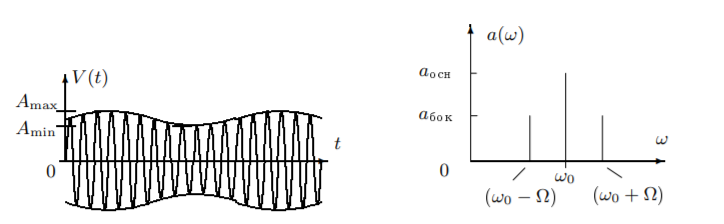
\includegraphics[width=0.8\textwidth]{4.png} 
    \caption{Амплитудно-модулированные колебания и их спектр}
    \label{AMosc}
\end{figure}

Рассмотрим гармонические колебания высокой частоты $\omega_0$, амплитуда которых медленно меняется по гармоническому закону с частотой $\Omega \ll \omega_0$ (см. рис. \ref{AMosc}).

\begin{equation}
    f(t) = A_0 \left[1+m\cos \Omega t\right] \cos \omega_0 t.
    \label{AMequation}
\end{equation}

Коэффициент $m$ - глубина модуляции. При $m < 1$ амплитуда меняется от минимальной $A_{\text{min}} = A_0(1 - m)$ до максимальной $A_{\text{max}} = A_0(1 + m)$. Глубина модуляции может быть представлена в виде

\begin{equation}
    m = \dfrac{A_{max} - A_{min}}{A_{max} + A_{min}}.
\end{equation}

Преобразовав уравнение \eqref{AMequation}, можно найти спектр колебаний:

\begin{equation}
    f(t) = A_0 \cos \omega_0 t + \dfrac{A_0 m}{2} \cos \left(\omega_0 + \Omega\right)t + \dfrac{A_0 m}{2}\cos\left(\omega_0 - \Omega\right)t.
\end{equation}

\subsection{Экспериментальная установка}

\begin{figure}[h]
    \centering
    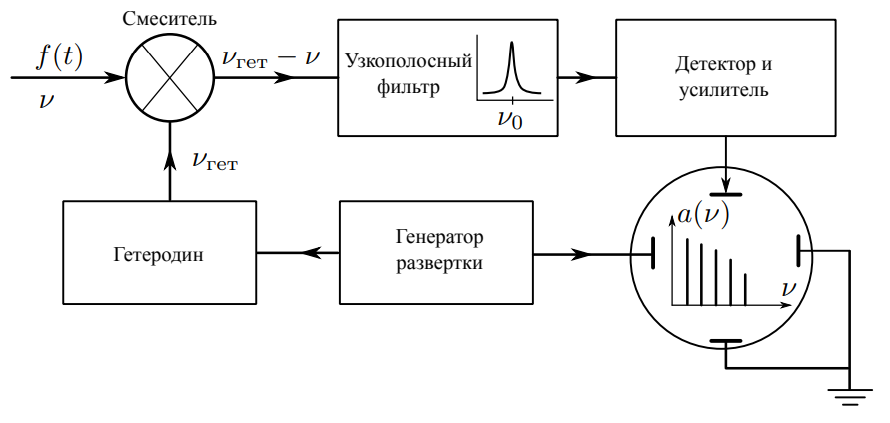
\includegraphics[width=0.8\textwidth]{setup.png} 
    \caption{Структурная схема анализатора спектра}
    \label{setup}
\end{figure}

Схема анализатора спектра, использованного в данной работе, изображена на рис. \ref{setup}. Исследуемый сигнал $f(t)$ и синусоидальный сигнал от вспомогательного генератора --- гетеродина --- подаются на вход смесителя. Смеситель — элемент, преобразующий колебания с частотами $\nu_1$ и $\nu_2$ в колебания на комбинированных частотах: $\nu_1 + \nu_2$ и $\nu_1 - \nu_2$. «Разностный» сигнал смесителя поступает на фильтр --— высокодобротный колебательный контур, настроенный на некоторую фиксированную резонансную частоту $\nu_0$. Таким образом, если $f(t)$ содержит гармонику $\nu = \nu_\text{гет} - \nu_0$ ($\nu_\text{гет}$ —-- частота гетеродина), она будет усилена, а отклик будет пропорционален её амплитуде.

В спектральном анализаторе частота гетеродина пропорциональна напряжению, подаваемому на развёртку по оси $X$ встроенного в анализатор осциллографа. Выходной сигнал подаётся на канал $Y$. На экране анализатора возникает, таким образом, график, изображающий зависимость амплитуды гармоник исходного сигнала от частоты, т. е. его спектр (при этом информация о фазах гармоник теряется).

В данной работе используемый цифровой осциллограф позволяет проводить электронную обработку сигналов и получить спектральный состав сигнала численно. Для этого используется алгоритм Быстрого преобразования Фурье (FFT).

\section{Оборудование и инструментальные погрешности.}

\textbf{В работе использовались:} генератор сигналов произвольной формы, цифровой осциллограф с функцией быстрого преобразования Фурье.

\textbf{Инструментальные погрешности:}

\begin{itemize}
    \item Генератор: относительная погрешность измерения характеристик колебаний $\varepsilon = 1 \%$;
    \item Курсоры осциллографа: погрешность - половина цены деления.
\end{itemize}

\section{Результаты измерений и обработка экспериментальных данных}

\subsection{Исследование спектра периодической последовательности прямоугольных импульсов}

Спектры сигналов при различных $\nu$ и $\tau$ представлены на рис. \ref{tab:picsI}.

\begin{table}[ht]
\begin{tabular}{ccc}
\begin{subfigure}{0.3\textwidth}\centering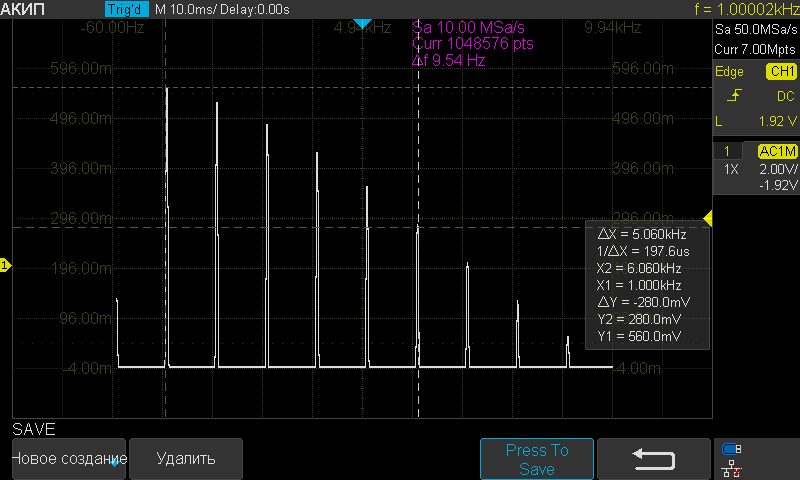
\includegraphics[width=\columnwidth]{I/AKIP0006.png}\caption{$\nu = 1$ кГц, $\tau = 100$ мс}\end{subfigure} &
\begin{subfigure}{0.3\textwidth}\centering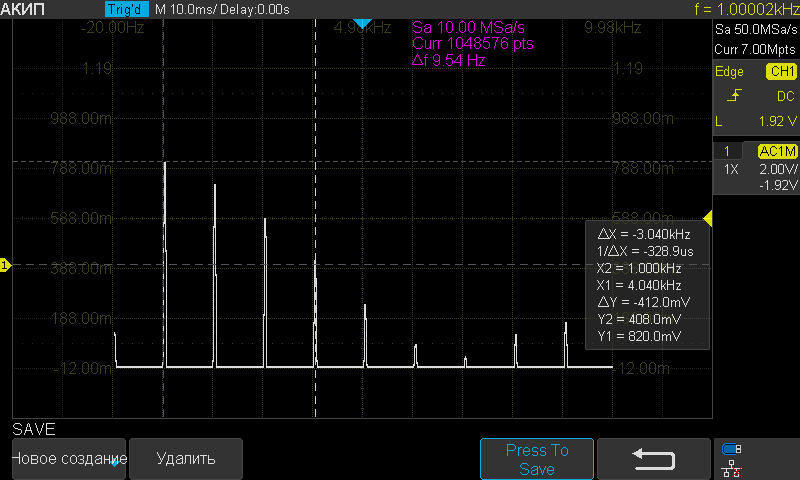
\includegraphics[width=\columnwidth]{I/AKIP0007.png}\caption{$\nu = 1$ кГц, $\tau = 150$ мс}\end{subfigure} &
\begin{subfigure}{0.3\textwidth}\centering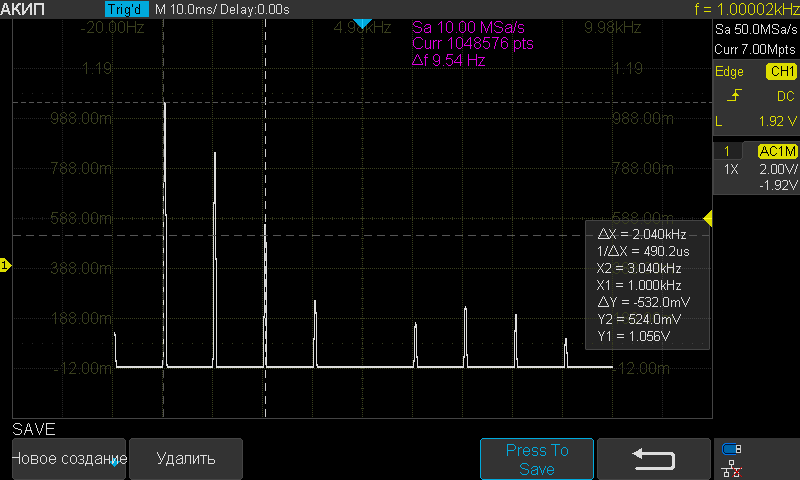
\includegraphics[width=\columnwidth]{I/AKIP0008.png}\caption{$\nu = 1$ кГц, $\tau = 200$ мс}\end{subfigure} \\
\newline
\begin{subfigure}{0.3\textwidth}\centering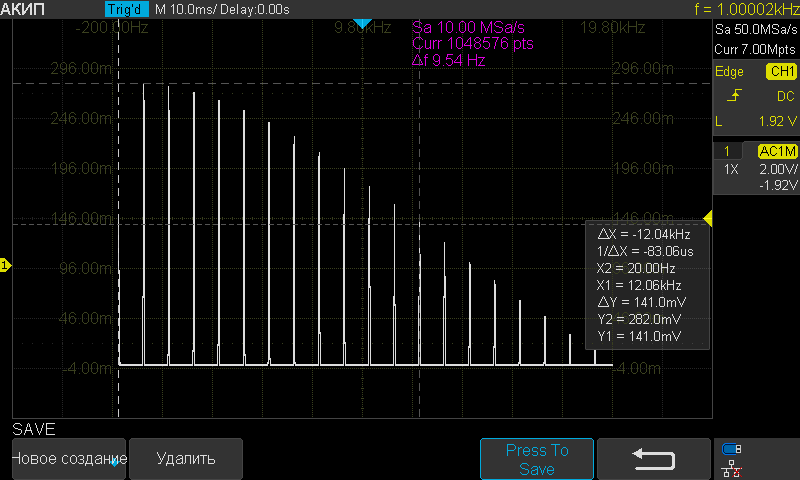
\includegraphics[width=\columnwidth]{I/AKIP0009.png}\caption{$\nu = 1$ кГц, $\tau = 50$ мс}\end{subfigure} &
\begin{subfigure}{0.3\textwidth}\centering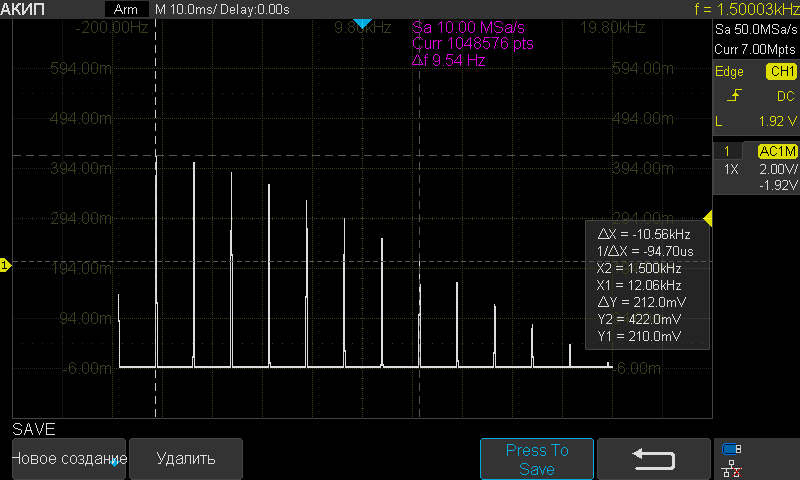
\includegraphics[width=\columnwidth]{I/AKIP0010.png}\caption{$\nu = 1,5$ кГц, $\tau = 50$ мс}\end{subfigure} &
\begin{subfigure}{0.3\textwidth}\centering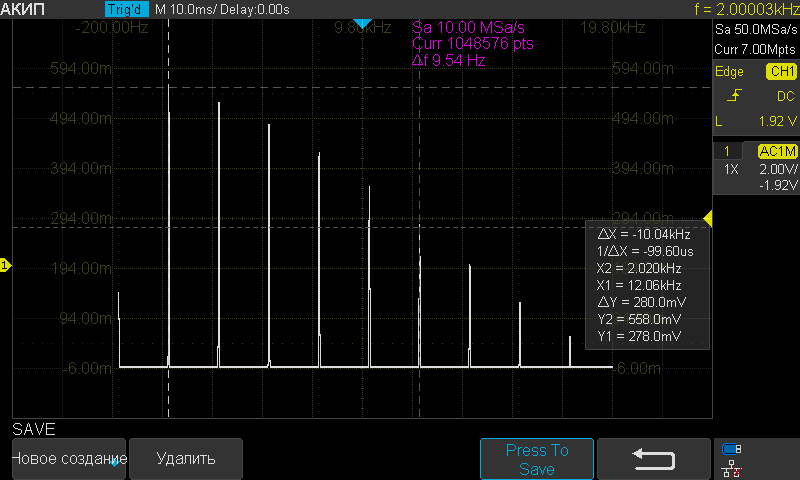
\includegraphics[width=\columnwidth]{I/AKIP0011.png}\caption{$\nu = 2$ кГц, $\tau = 50$ мс}\end{subfigure} \\
\end{tabular}
\caption{Спектр последовательности прямоугольных импульсов при разных значениях параметров}
\label{tab:picsI}
\end{table}

При фиксированных $\nu = 1$ кГц и $\tau = 150$ мкс были измерены амплитуды $a_n$ и частоты $\nu_n$ для первых 6 гармоник спектра. Рассчитанные и измеренные значения представлены в таб. \ref{tab:harmonicsI}. Для сравнения теоретически рассчитанной и измеренной амплитуд сделана нормировка по наименьшему значению.

\begin{table}[h!]
\begin{center}
\begin{tabular}{|c|c|c|c|c|c|}
\hline
$n$ & $\nu_{\text{теор}}$, кГц & $a_{\text{теор}}$, мВ & $\nu_{\text{изм}}, кГц$ & $a_{\text{изм}}$, мВ & $\Delta_a$, \% \\ \hline
1 & 1,00 & 881 & 1,02 & 824 & 6,5 \\ \hline
2 & 2,00 & 785 & 2,02 & 736 & 6,2\\ \hline
3 & 3,00 & 639 & 3,02 & 600 & 6,1 \\ \hline
4 & 4,00 & 462 & 4,02 & 432 & 6,5 \\ \hline
5 & 5,00 & 275 & 5,02 & 260 & 5,5 \\ \hline
6 & 6,00 & 100 & 6,04 & 102 & 2,0 \\ \hline
\end{tabular}
\end{center}
\caption{Теоретические и экспериментальные значения амплитуд и частот гармоник спектра}
\label{tab:harmonicsI}
\end{table}

Результаты измерений зависимости ширины спектра $\Delta{\nu}$ от времени импульса $\tau$ в диапазоне от 20 до 200 мкс при фиксированной $\nu = 1$ кГц представлены в таб. \ref{tab:resultsI}.

\begin{table}[h!]
\begin{center}
\begin{tabular}{|c|c|c|c|}
\hline
$\tau$, мкс & $1/\tau$, $10^3$ 1/c & $\Delta{\nu}, кГц$ \\ \hline
20 & 50 & 28,20 \\ \hline
50 & 20 & 12,00 \\ \hline
100 & 10 & 5,00 \\ \hline
150 & 6,6 & 3,04  \\ \hline
200 & 5 & 2,04 \\ \hline
\end{tabular}
\end{center}
\caption{Зависимость ширины спектра $\Delta{\nu}$ от длительности импульса $\tau$}
\label{tab:resultsI}
\end{table}

График зависимости $\Delta{\nu}(1/\tau)$ представлен на рис. \ref{plotI}. Получена линейная зависимость, что удовлетворяет соотношению неопределённостей.

\begin{figure}[h!]
\centering
\resizebox {0.55\textwidth} {!} {
\begin{tikzpicture}
\begin{axis}[ xlabel = {$1/\tau$, $10^3$ c$^{-1}$}, ylabel = {$\Delta\nu$, кГц}, xmin = 0, xmax = 60, ymin = 0, ymax = 35, minor tick num = 5]
\addplot[color=black, mark=x, only marks] coordinates{
(5, 2.04)
(6.6, 3.04)
(10, 5)
(20, 12)
(50, 29.2)
};
\addplot[color=blue, domain=0:55] {0.59*x};
\end{axis}
\end{tikzpicture}
}
\caption{График зависимости ширины спектра $\Delta{\nu}$ от длительности импульса $\tau$}
\label{plotI}
\end{figure}

\subsection{Исследование спектра периодической последовательности цугов}

Спектры сигналов при различных $\nu_0$, $T$ и $N$ представлены в таблице. .

\begin{table}[ht]
\begin{tabular}{ccc}
\begin{subfigure}{0.3\textwidth}\centering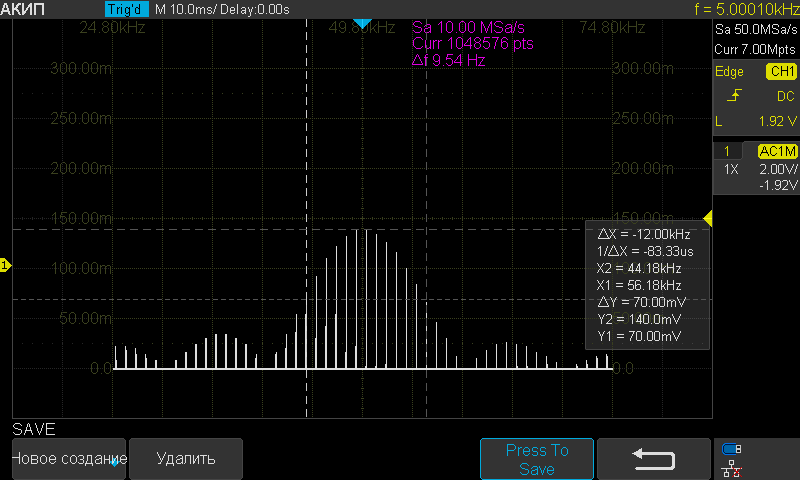
\includegraphics[width=\columnwidth]{II/AKIP0012.png}\end{subfigure} &
\begin{subfigure}{0.3\textwidth}\centering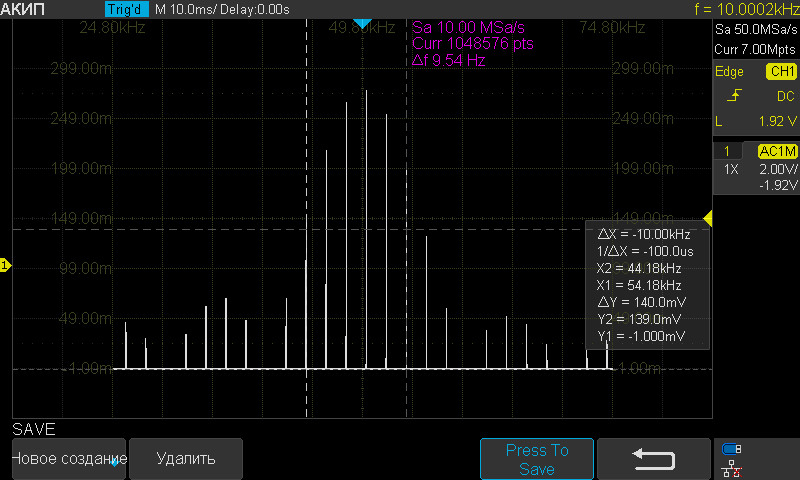
\includegraphics[width=\columnwidth]{II/AKIP0013.png}\end{subfigure} &
\begin{subfigure}{0.3\textwidth}\centering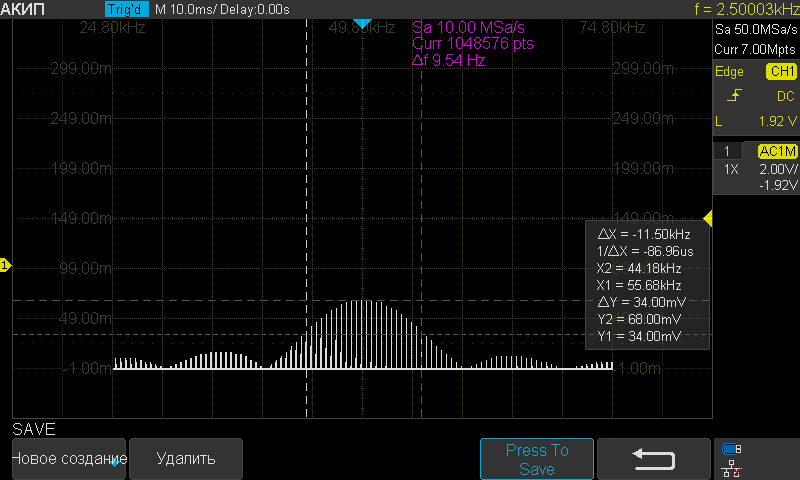
\includegraphics[width=\columnwidth]{II/AKIP0014.png}\end{subfigure} \\
\newline
\begin{subfigure}{0.3\textwidth}\centering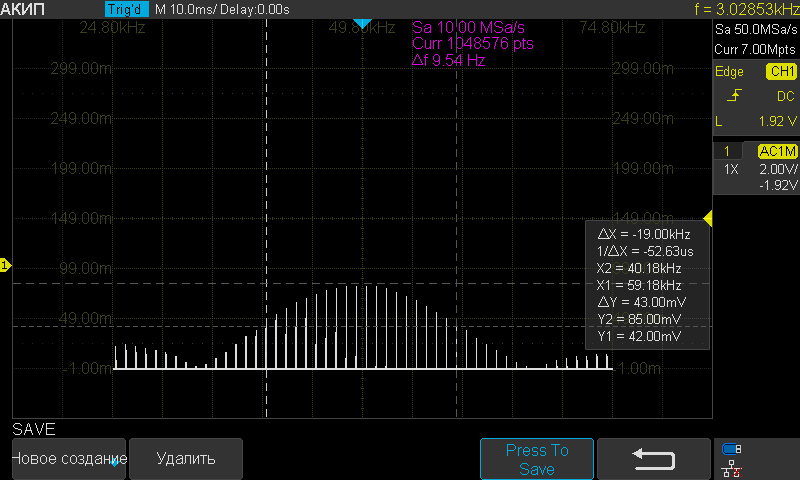
\includegraphics[width=\columnwidth]{II/AKIP0015.png}\end{subfigure} &
\begin{subfigure}{0.3\textwidth}\centering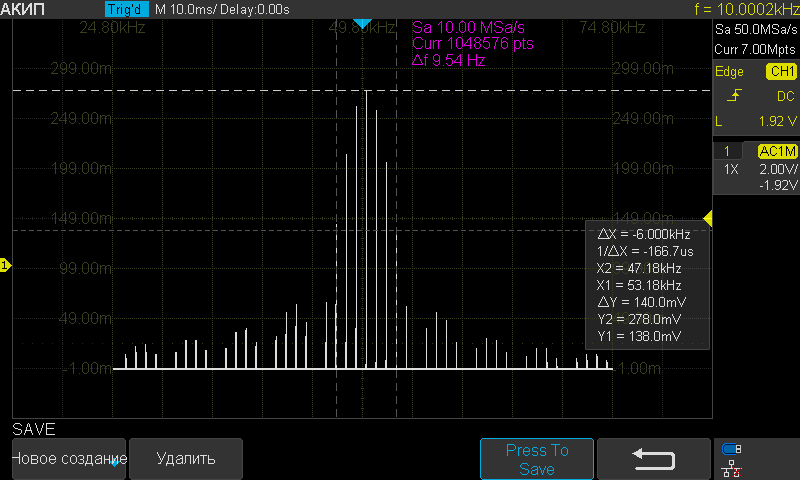
\includegraphics[width=\columnwidth]{II/AKIP0016.png}\end{subfigure} &
\begin{subfigure}{0.3\textwidth}\centering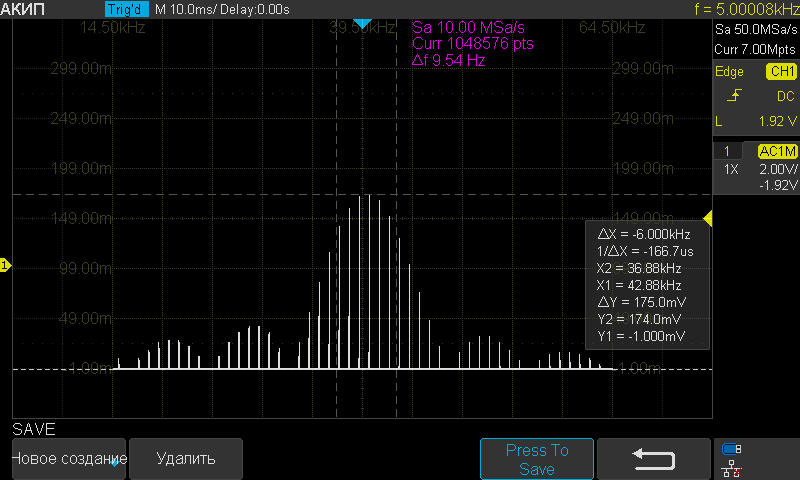
\includegraphics[width=\columnwidth]{II/AKIP0017.png}\end{subfigure} \\
\end{tabular}
\caption{Спектр периодической последовательности цугов при разных значениях параметров}
\label{tab:picsII}
\end{table}

При фиксированных параметрах $\nu_0 = 50$ кГц и $N = 5$ была измерена зависимость расстояния $\delta\nu$ между соседними спектральными компонентами сигнала от периода $T$ повторения импульсов в диапазоне $T = 0,5 - 2,5$ мс. Измеренные значения представлены в таб. \ref{tab:resultsII}.

\begin{table}[h!]
\begin{center}
\begin{tabular}{|c|c|c|}
\hline
$T, мс$ & $1/T$, $10^3$ c$^{-1}$ & $\delta\nu, кГц$ \\ \hline
0,5 & 2,0 & 2,0 \\ \hline
1,0 & 1,0 & 1,0 \\ \hline
1,5 & 0,66 & 0,66 \\ \hline
2,0 & 0,5 & 0,5 \\ \hline
2,5 & 0,4 & 0,4 \\ \hline
\end{tabular}
\end{center}
\caption{Результаты измерений зависимости $\delta\nu(T)$}
\label{tab:resultsII}
\end{table}

Полученный график зависимости $\delta{\nu}(1/T)$ представлен на рис.\ref{plot2}. Коэффициент наклона равен 1 в пределах инструментальной погрешности.

\begin{figure}[h!]
\centering
\resizebox {0.55\textwidth} {!} {
\begin{tikzpicture}
\begin{axis}[ xlabel = {$1/T$, $10^3$ c$^{-1}$}, ylabel = {$\delta\nu$, кГц}, xmin = 0, xmax = 2.5, ymin = 0, ymax = 2.5, minor tick num = 5]
\addplot[color=purple, mark=x] coordinates{
(0, 0)
(0.4, 0.4)
(0.5, 0.5)
(0.66, 0.66)
(1.0, 1.0)
(2.0, 2.0)
};
\end{axis}
\end{tikzpicture}
}
\caption{График зависимости расстояния между гармониками $\delta{\nu}$ от периода $1/T$}
\label{plotII}
\end{figure}

\subsection{Исследование спектра амплитудно-модулированного сигнала}

Спектр амплитудно-модулированного сигнала при разных значениях $\nu_0$ и $\nu$ представлен на рис. \ref{tab:picsIII}.

\begin{table}[ht]
\begin{tabular}{ccc}
\begin{subfigure}{0.3\textwidth}\centering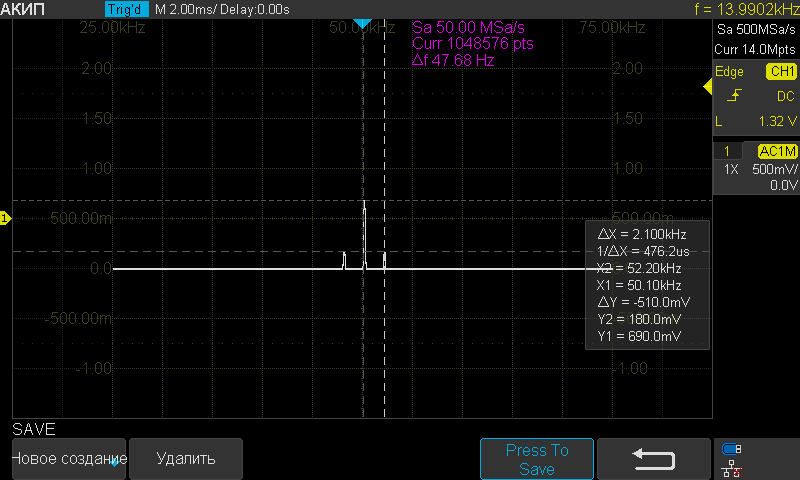
\includegraphics[width=\columnwidth]{III/AKIP0018.png}\end{subfigure} &
\begin{subfigure}{0.3\textwidth}\centering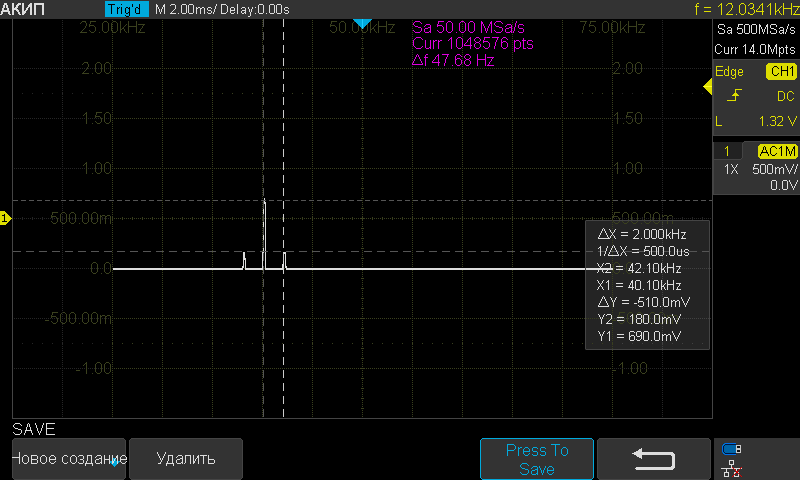
\includegraphics[width=\columnwidth]{III/AKIP0019.png}\end{subfigure} &
\begin{subfigure}{0.3\textwidth}\centering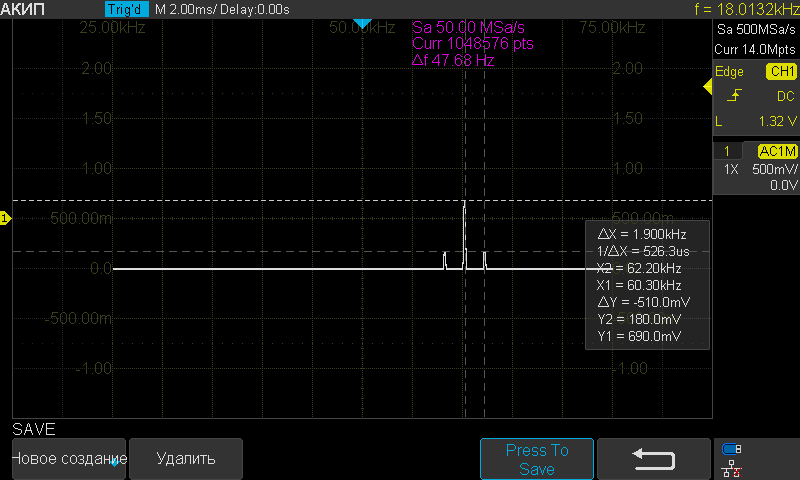
\includegraphics[width=\columnwidth]{III/AKIP0020.png}\end{subfigure} \\
\newline
\begin{subfigure}{0.3\textwidth}\centering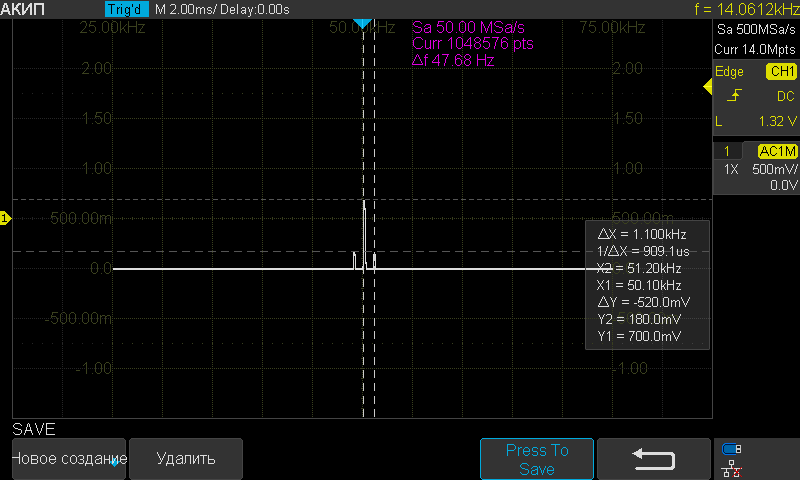
\includegraphics[width=\columnwidth]{III/AKIP0022.png}\end{subfigure} &
\begin{subfigure}{0.3\textwidth}\centering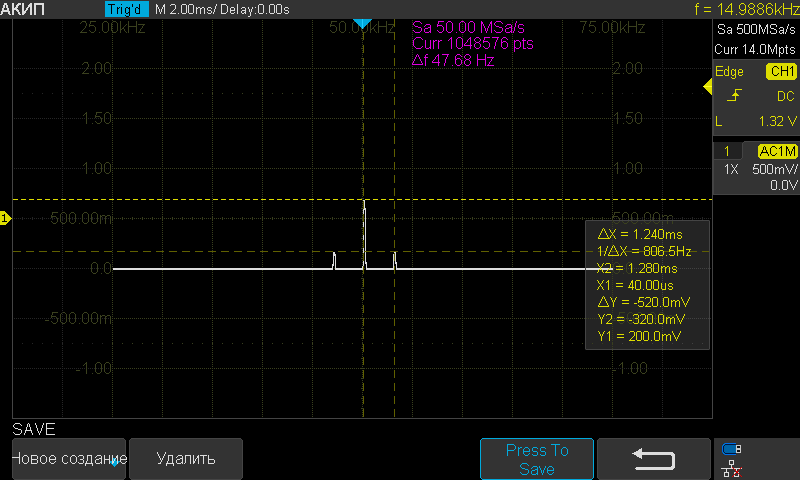
\includegraphics[width=\columnwidth]{III/AKIP0023.png}\end{subfigure} &
\begin{subfigure}{0.3\textwidth}\centering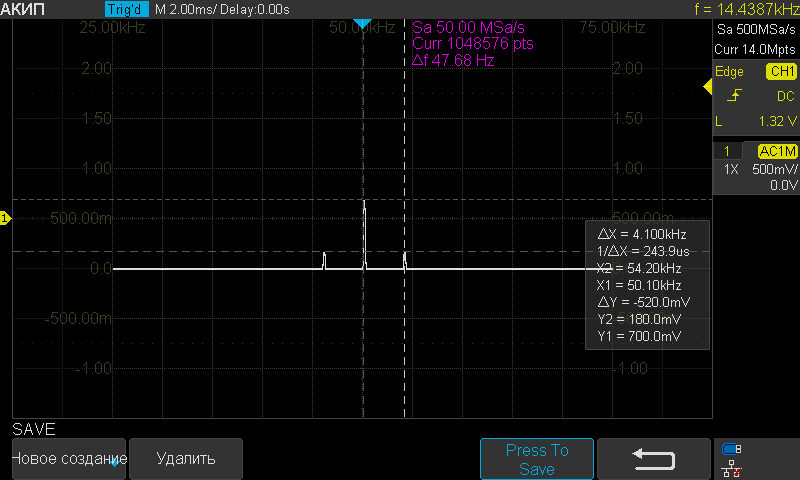
\includegraphics[width=\columnwidth]{III/AKIP0024.png}\end{subfigure} \\
\newline
\begin{subfigure}{0.3\textwidth}\centering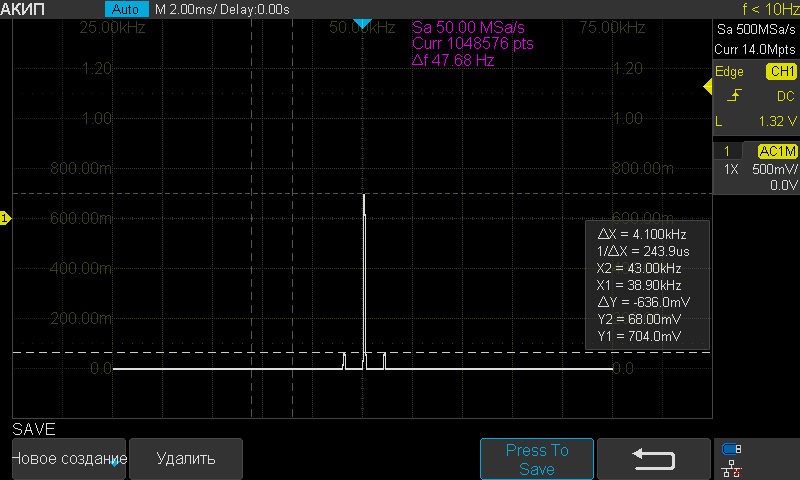
\includegraphics[width=\columnwidth]{III/AKIP0025.png}\end{subfigure} &
\begin{subfigure}{0.3\textwidth}\centering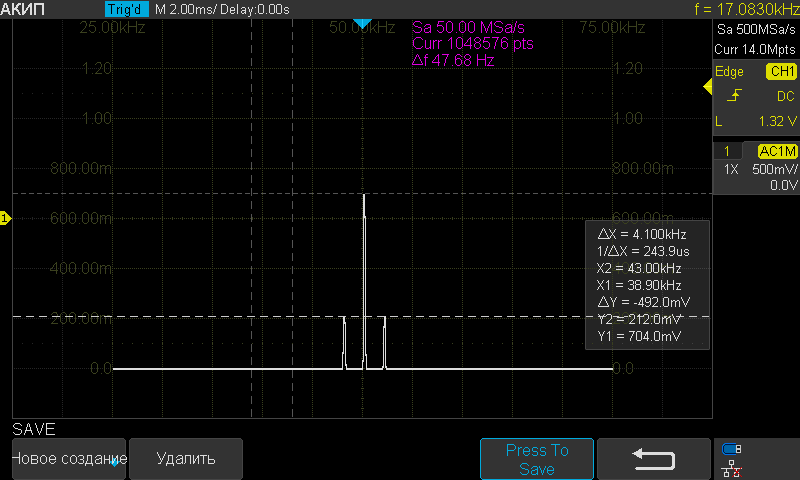
\includegraphics[width=\columnwidth]{III/AKIP0026.png}\end{subfigure} &
\begin{subfigure}{0.3\textwidth}\centering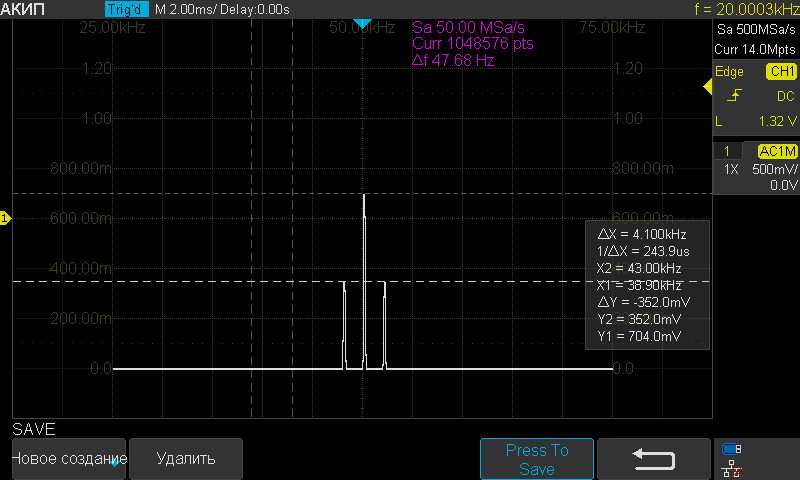
\includegraphics[width=\columnwidth]{III/AKIP0027.png}\end{subfigure} \\
\end{tabular}
\caption{Спектр амплитудно-модулированного сигнала при разных значениях параметров}
\label{tab:picsIII}
\end{table}

Для проверки правильности измерений была вычислена и измерена напрямую величина $m$:

\begin{itemize}
    \item $m = 0,5$;
    \item $m = (A_{max} - A_{min})/(A_{max} + A_{min}) = \frac{1,52 - 0,51}{1,52 + 0,51} \approx 0,5$.
\end{itemize}

Равенство справедливо в пределах погрешности измерений.

При фиксированных параметрах $\nu_0 = 60$ кГц и $\nu_{мод} = 5$ кГц была измерена зависимость отношения $a_\text{бок}/a_\text{осн}$ амплитуд боковой и основной спектральных линий от глубины модуляции $m$  в диапазоне от 10\% до 100\%. Измеренные значения представлены в таб. \ref{tab:resultsIII}.

\begin{table}[h!]
\begin{center}
\begin{tabular}{|c|c|c|c|c|c|c|}
\hline
$m$ & $a_\text{бок}$, мВ & $a_\text{осн}$, мВ & $a_\text{бок}/a_\text{осн}$ \\ \hline
0,1 & 36 & 704 & 0,051 \\ \hline
0,2 & 68 & 704 & 0,096 \\ \hline
0,3 & 108 & 704 & 0,153 \\ \hline
0,4 & 140 & 704 & 0,199 \\ \hline
0,5 & 172 & 704 & 0,244 \\ \hline
0,6 & 212 & 704 & 0,301 \\ \hline
0,7 & 244 & 704 & 0,347 \\ \hline
0,8 & 276 & 704 & 0,392 \\ \hline
0,9 & 316 & 704 & 0,449 \\ \hline
1,0 & 352 & 704 & 0,500 \\ \hline
\end{tabular}
\end{center}
\caption{Результаты измерений зависимости $a_\text{бок}/a_\text{осн}$ от $m$}
\label{tab:resultsIII}
\end{table}

Полученный график зависимости зависимости $a_\text{бок}/a_\text{осн}$ от $m$ представлен на рис. \ref{plotIII}. Коэффициент наклона прямой равен 0,5 в пределах инструментальной погрешности.

\begin{figure}[h!]
\centering
\resizebox {0.55\textwidth} {!} {
\begin{tikzpicture}
\begin{axis}[ xlabel = {$m$}, ylabel = {$a_\text{бок}/a_\text{осн}$}, xmin = 0, xmax = 1.1, ymin = 0, ymax = 0.55, minor tick num = 5]
\addplot[color=black, mark=x, only marks] coordinates{
(0.1, 0.051)
(0.2, 0.096)
(0.3, 0.153)
(0.4, 0.199)
(0.5, 0.244)
(0.6, 0.301)
(0.7, 0.347)
(0.8, 0.392)
(0.9, 0.449)
(1, 0.5)
};
\addplot[color=red] {0.5*x};
\end{axis}
\end{tikzpicture}
}
\caption{График зависимости отношения амплитуд боковой и основной гармоник от глубины модуляции $m$}
\label{plotIII}
\end{figure}

\section{Обсуждение результатов и выводы}

В данной работе были успешно вычислены спектры следующих сигналов: последовательности прямоугольных импульсов, последовательности цугов и амплитудно-модулированного сигнала. Все измеренные спектры качественно совпадают с теоретическими, что говорит о правильности работы цифрового осциллографа и БПФ. 

Погрешности при измерении спектров последовательности цугов и амплитудно-модулированного сигнала минимальны и сравнимы по величине с инструментальными, которые также очень малы по сравнению с измеренными величинами. Об этом говорит видимое отсутствие отклонений измеренных линейных зависимостей от теоретических. Погрешность при измерении полуширины спектра последовательности прямоугольных импульсов несколько больше, так как по дискретному набору точек нельзя прямо (с помощью измерительных приборов) определить полуширину кривой, через них проходящей. Однако незначительность погрешности ($> 10\%$) позволяет установить линейность зависимости, что соответствует теоретической оценке. Погрешность определения величин гармоник спектра не превосходит 7\%, что также позволяет говорит о высокой точности измерений.    

\end{document}
